Au début de mon stage, le projet ayant un an, les fonctionnalités développées ci-dessous était déjà développer. J'ai cependant intervenus
sur la pluspart d'entre elles soit pour des corrections de bugs d'une part, soit à des fin d'améliorations d'autres part.

Afin de présenter mon travail que vous trouverez chapitre \ref{collaboration}, il est nécessaire de présenter le fonctionnement général de
cette plateforme afin d'en avoir une vue d'ensemble.

	\section{Le fichier Walkthrough}\label{wt}
		Le fichier Walkthrough est un fichier qui sera fourni par la personne en charge des tests, c'est un fichier au format Excel qui contient les informations
		de chacune des variables à tester. Il contient ainsi un très grand nombre de colonnes, bien que seule une partie des colonnes nous
		intéresse, certaines colonnes ont été remplies par le fournisseur du plugin, d'autres colonnes sont ajoutées dans le seul but de la
		génération de tests automatiques par \textit{GreenT}. Voici les colonnes les plus intéressantes : 

		\begin{description} 
			\item[Nom de la variable] Le nom de la variable testée : il existe un nom court et un nom long.
			\item[Informations aidant à la conversion des données] Certains \textit{devices} tel que le debugger ne fonctionne qu'avec des
				valeurs Hexadécimales. À la charge de \textit{GreenT} de convertir ces données vers des valeurs physiques exploitables par
				le testeur. Ces colonnes contiennent les informations nécessaires au calcul de conversion\footnote{Informations tel que le
				domaine de définition physique et le domaine de définition hexadécimal}.
			\item[Nécessité d'un test automatique] un \texttt{GreenTTest} ne sera généré que si la colonne vaut \textit{Yes}.
			\item[Statut du test] Nous éditerons cette colonne afin de reporter le statut du test\footnote{Un test pouvant être Green ou Red
				mais peut aussi comporter une erreur, tel qu'un problème d'exécution ou de génération, \ldots}.
			\item[Precondition (cf section \ref{stim})] Contient un scénario d'initialisation du \textit{workbench} : tension de départ,
				démarrage de l'ECU, \ldots
			\item[Scénario de stimulation (cf section \ref{stim})] Contient un ou plusieurs scénarios de stimulations
			\item[\texttt{ExpectedBehavior} (comportement attendu, cf section \ref{expectedBehavior})] Contient une expression évaluant les variables ayant été enregistrées durant la stimulation : \textit{GreenT} devra vérifier que cette expression est correct à toute instant de la stimulation.
			\item[Variable à enregistrer (cf section \ref{expectedBehavior})] Contient les variables devant être enregistrées durant un
				scénario, en plus des variables présentes dans l'expected behavior. Celles-ci peuvent servir en tant que données
				contextuelles permettant de mieux cerner le résultat d'un test.
			\item[Alias locaux (cf section \ref{alias})] Ce sont des alias déclarés uniquement pour le test courant.
			\item[Informations du test (cf section \ref{report})] Plusieurs colonnes tel que la sévérité, le responsable du test, les commentaires, \ldots
		\end{description}

		\begin{figure}[H]
			\centering
			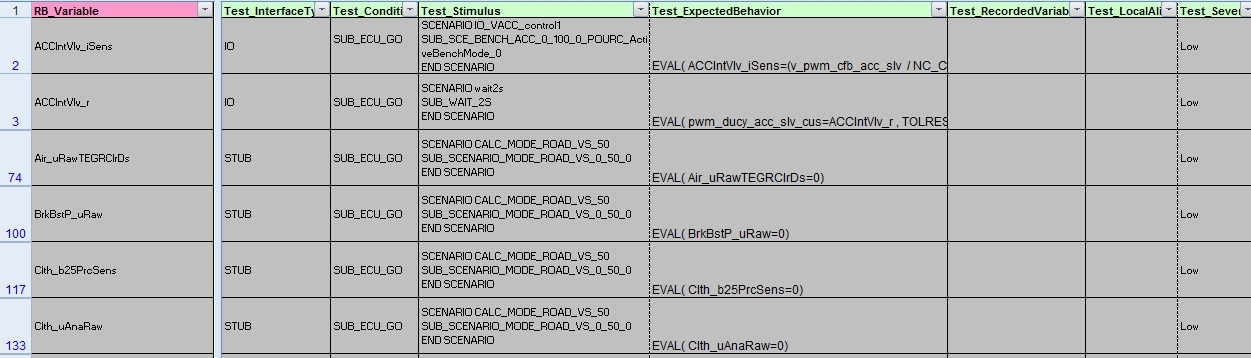
\includegraphics[width=18.5cm]{contents/images/walkthrough.png}
			\caption{Aperçu d'un fichier Walkthrough}
		\end{figure}
		\section{Fonctionnement Global}
	Le développement de \textit{GreenT} inclu un certain nombre de fonctionnalités attendues par le client et indispensable à son fonctionnement. D'autres fonctionnalités pourront apparaître plus tard en fonction des besoins.

	Les principaux modules sont les suivants, avec leurs interactions schématisées figure \ref{fig:generalDiag} : 
			Dans des objets ovales sont représentés des fichiers, les carrés représentent des modules de la plateforme et les flèches en pointillés un transfert réseau, les couleurs représentent les différents modules de la plateforme.

		\begin{figure}[H]
			\centering
			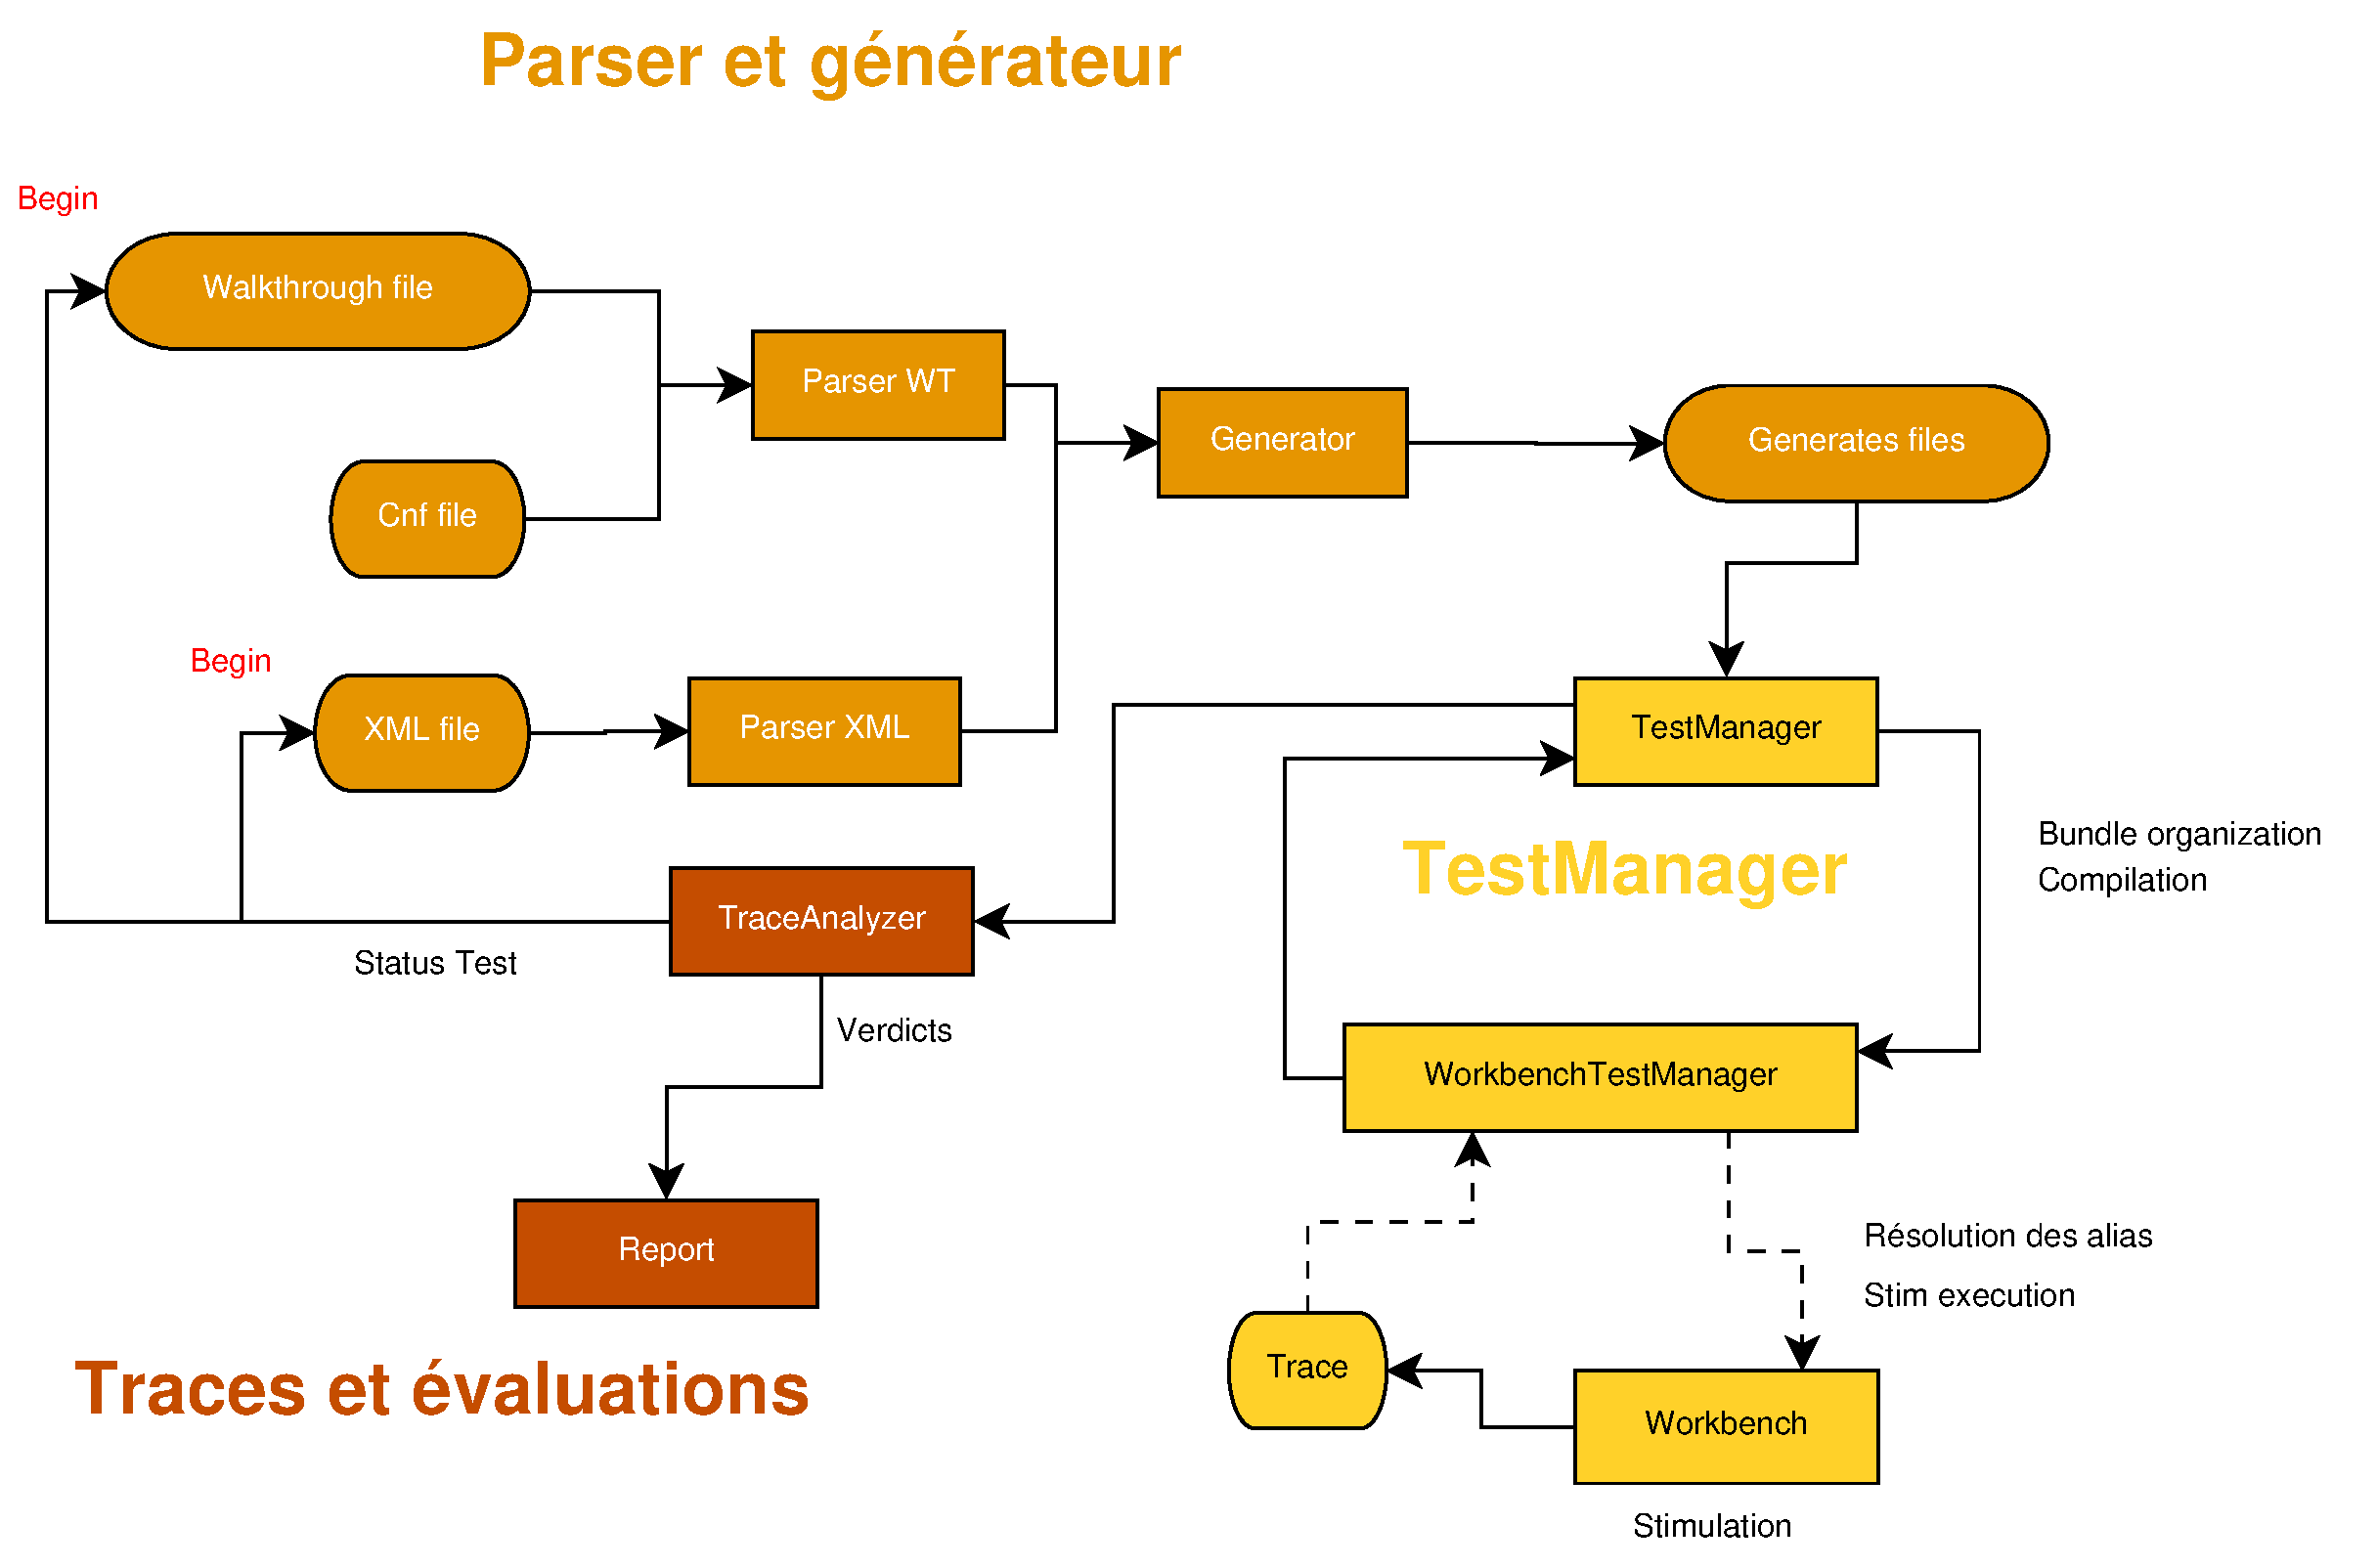
\includegraphics[width=16.5cm]{contents/images/generalDiag.eps}
			\caption{Fonctionnement général de la plateforme \textit{GreenT}}
			\label{fig:generalDig}
		\end{figure}	

		Dans la figure \ref{fig:generalDig}, vous pouvez voir des flèches en pointillés représentant des échanges réseau. En effet
		l'exécution des stimulations et l'enregistrement des traces se fait par un contrôle distant des bancs de tests\footnote{La
		schématisation du fonctionnement d'un banc est disponible section \ref{chapPb} figure \ref{fig:photoHil}}.

		Les principales fonctionnalités demandées par le client sont disponibles sur le client, la majorité peuvent s'effectuer en local : 
		\begin{itemize}
			\item Le parsing et la génération (section \ref{generation})
			\item L'organisation en Bundle (section \ref{testManager})
			\item La production de rapports détaillés (section \ref{expectedBehavior})
		\end{itemize}~\newline
		Alors que d'autres fonctionnalités vont nécessiter la présence de serveurs et de connexion réseau permettant d'effectuer ces actions
		: 
		\begin{itemize}
			\item Les stimulations (section \ref{stim})
			\item Les enregistrement des traces (section \ref{stim})
		\end{itemize}

		\section{Les différentes fonctionnalités du Client, GreenT}
		Afin de répondre au mieux aux attentes du client, il a été choisi d'utiliser le Java pour développer notre client, ceci en raison de
		diverses avantages comme le côté multi-plateforme, son typage fort et sa forte communauté qui permet ainsi une maintenance réduite. 

	\subsection{Parsing et Génération}\label{generation}
	Le but premier de la plateforme est d'effectuer des tests automatiques, il est ainsi indispensable d'avoir un système d'automatisation.

	Pour cela, nous avons un parser : il analyse un certain type de fichier\footnote{Nous ne commencerons qu'avec le Walkthrough pour débuter, mais dans le futur nous pourrions avoir des fichiers XML, des bases de données, \ldots} et en retire pour chaque test, le scénario de pré condition, les différents scénarios de stimulations, leurs \textit{Expected Behavior}, les données qui devront être enregistrées ainsi que différentes information sur le test\footnote{Responsable du test, sévérité, commentaires, nom de la variable, \ldots}.

	Une fois toutes ces données acquises, il les transmet à un générateur qui est en charge d'écrire les fichiers Java de chaque test, tous sont organisés dans un dossier temporaire avec un dossier par test. Le \texttt{TestManager} peut ensuite traiter ces données.

	\subsection{Stimulation} \label{stim}
		Afin de tester une variable du plugin, les développeurs vont utiliser des alias présents sur un device : actuellement, un HIL ou un debugger, prochainement nous pourrions en utiliser d'autres que ces deux derniers.

		Le spécifieur va rédiger des scénarios de stimulation, ceci afin de mettre le contrôleur dans certaines conditions. Son but sera ensuite de vérifier que ces variables restent cohérentes vis-à-vis du scénario effectué. 

		Un scénario particulier doit être spécifié : une pré condition qui a pour but d'initialiser les \textit{devices} et certains alias afin d'avoir un état de stimulation qui soit cohérent et identique à chaque lancement du scénario. Ce scénario sera effectué avant le lancement de chacun des scénarios de stimulation.

		Durant l'exécution d'une stimulation, les variables nécessaires sont enregistrées afin de pouvoir produire des rapports et des
		verdicts ensuite.

	\subsection{Les traces et leurs évaluations}\label{expectedBehavior}
	Lorsqu'un scénario de stimulation s'exécute, un certain nombre de variables sont enregistrées : ces variables sont stockées sous la forme d'une trace au format CSV, qui pourra plus tard être représentée sous forme de courbe. 

	Une fois que la trace est complète, il est nécessaire de l'évaluer : le spécifieur a décrit le comportement attendu dans la colonne \textit{Expected Behavior} détaillant dans quel cas le test est correct, ainsi cette expression va être transformée en arbre logique afin de l'évaluer à tout instant de la trace. 

\subsection{Le module TestManager}\label{testManager}
	Le \texttt{TestManager} est le chef d'orchestre de \textit{GreenT}, il a donc un certain nombre de responsabilités. 

	Il va d'abord organiser les différents tests en un concept que nous avons appelé \textit{Bundle} : afin de limiter le temps d'exécution qui atteindra plusieurs dizaines d'heures, il est intéressant de regrouper les tests possédant les mêmes scénarios de stimulations et les mêmes pré conditions. Seules leur \textit{Expected Behavior} changent, mais celles-ci pourront être évaluées sur la même Trace.

	Une fois les tests organisés en \textit{Bundle}, il va les compiler et les donner à un \texttt{WorkbenchManager} : toujours pour une
	raison d'optimisation, il sera intéressant de pouvoir exécuter les enregistrements sur plusieurs bancs simultanément, pour cela le
	\texttt{TestManager} sera capable de savoir quels bancs peuvent être utilisés et pourra distribuer ses \textit{bundles} en fonction. 

	Chaque \texttt{WorkbenchManager} sera en charge d'exécuter le code généré plus tôt et dialoguera en réseau avec son banc, une fois l'exécution terminée, il obtiendra une trace qui pourra être évaluée.

	Afin d'être le plus souple possible, il existe plusieurs modes d'exécution du \texttt{TestManager} : 
	\begin{description}
		\item[Check only] Essaye de parser les différents fichiers, et vérifie que ceux-ci ne comportent aucune erreur de grammaire, d'alias introuvable, d'écriture sur un alias en lecture seule etc...
		\item[Parse and generate bundles] Parse les fichiers et génère des jars exécutables répartis en bundle
		\item[Parse and execute] Parse les fichiers, génère les jars pour les bundles et les exécute : c'est le mode << classique >>.
		\item[Restart test execution] Redémarre une exécution qui se serait mal terminée.
	\end{description}

	\subsection{Production de rapport détaillé}\label{report}
	La plateforme a en charge la production d'un rapport détaillé pour chaque test. Ce rapport contiendra un certain nombre d'informations, et permettra au testeur de comprendre pourquoi le test n'est pas passé. Voici les informations que contiendra ce rapport : 

	\begin{itemize}
		\item Nom du test, de la variable à tester
		\item Nom du responsable du test
		\item Sévérité du test
		\item Pourcentage de branches de l'expectedBehavior renvoyant faux(Test << Rouge >>), n'ayant pas pu être testé(Test << Gris >>) et étant correct(Test Vert)
		\item Le testeur aura à sa disposition les expressions concernées par un résultat Rouge ou Gris.
		\item Les colonnes utiles du \texttt{Walkthrough}
	\end{itemize}

	Actuellement, les rapports se font au format Excel avec l'intégralité de notre enregistrement et pour chaque timestamp, un verdict. Un
	exemple de rapport est accessible en Annexe TODO page TODO. 
	% TODO TODO TODO TODO Add report in appendix 
	
	Dans un futur proche, ces rapports pourraient être générés dans un format Web avec une possibilité de naviguer entre plusieurs tests, et
	d'avoir un affichage des courbes de manière graphique.

	\subsection{Mise à jour du Walkthrough}
	Une fois un test exécuté, un résultat est mis dans le fichier Excel, en fonction de l'analyse précédemment de la trace : un verdict rouge renverra un résultat rouge, si tout est vert le résultat vert et enfin, celui-ci pourra être gris si nous n'avons pas été capable d'evaluer de résultats.


	\section{Fonctionnement des serveurs}
	Comme expliqué précédemment, GreenT va avoir en charge l'exécution de stimulation. Ces stimulations vont communiquer avec une table de
	tests. Actuellement une table est composée de deux \textit{devices} différents, comportant chacun leur serveur : 
	\begin{itemize}
		\item Un HIL, Hardware In the Loop, simulateur d'environnement véhicule
		\item Un Debugger permettant de voir l'état du programme présent dans l'ECU
	\end{itemize}

	Au début du développement de la plateforme, il a été décidé que les serveurs devront être le plus simple possible pour plusieurs raisons
	: 
	\begin{itemize}
		\item Rabattre le maximum de fonctionnement métier près du client pour centraliser au maximum le fonctionnement et éviter la
			maintenance superflue
		\item Avoir la possibilité de réutiliser les serveurs pour d'autres projets
		\item Pouvoir ajouter facilement un nouveau device, qui ne nécessiterai que l'ajout d'un nouveau serveur relativement simple
	\end{itemize}
	
	\subsection{Le serveur Debugger, Trace32}
	Le serveur Debugger propose des services basiques permettant de répondre aux différentes stimulations : 
	\begin{itemize}
		\item Mettre l'ECU à on
		\item Arrêter l'ECU
		\item Lire une variable ou une calibration
		\item Modifier une variable
		\item Enregistrer des variables
	\end{itemize}

	Afin d'effectuer ces actions, le serveur s'appuie sur une API fournie par l'outil Trace32 permettant de contrôler le debugger. Ainsi
	tous nos services vont s'appuyer sur cette API. C'est pour cette raison que ce serveur est développé en Java afin de pouvoir utiliser
	facilement ces fonctions.

	\subsection{Le serveur HIL, DSpace}
	Le serveur DSpace va devoir lui aussi répondre aux différentes stimulations, ainsi ces services sont relativement similaire : 
	\begin{itemize}
		\item Modifier une valeur de la base de données
		\item Lire une valeur de la base de données
		\item Enregistrer des valeurs
	\end{itemize}

	Ce serveur a été développé en réutilisant une partie de ce qui avait été fait pour la TA3, présenté section \ref{ta3} afin de ne pas
	<< réinventer la roue >>. À l'instar du serveur Debugger, nous utilisons une api fournie par l'outil permettant de contrôler le HIL : ControlDesk. 
	C'est ainsi que ce serveur est développé en Python afin de répondre à cette contraintes : l'API du ControlDesk est en Python.
	
